\chapter{Iunctura}\label{ch:03}

\begin{chapter_outline}

  We demonstrate the benefits of mixing distinct classes of probabilistic models. In particular, we study the complementary between variational autoencoders (VAEs) and denoising diffusion probabilistic models (DDPMs). While VAEs offer scalable amortised posterior inference and fast sampling, they are often outperformed by competing models such as normalizing flows (NFs) or deep-energy models. We improve VAEs by modelling the prior distribution of the latent variables with a diffusion process. The diffusion prior model improves upon Gaussian priors of classical VAEs and is competitive with NF-based priors.
  This contribution shows that connecting different classes of models can unlock modelling capacities and properties that are unreachable by each model class independently.
\end{chapter_outline}
\section{Prologue}
This chapter expresses the relevance of unifying the frameworks associated with distinct (deep) probabilistic models. Indeed, building a broad and deep understanding of different probabilistic modelling frameworks unlocks potential model combinations. These combinations may help reduce the weaknesses of each class of models separately while maintaining their assets. This is particularly relevant with deep probabilistic models for which the gradient-descent-based training framework allows jointly training all components of a `super` model if the objective function is a differentiable function of the model's components. We rely on this to combine denoising diffusion probabilistic models and variational autoencoders.

As will see in the paper, combining DDPMs and VAEs is pretty straightforward and leads to better modelling for image synthesis. We believe that further interplay between different probabilistic models is essential in developing tomorrow's probabilistic modelling toolbox. In an ideal world, combining two classes of deep probabilistic models should be as simple as replacing a Normal distribution with a Laplace distribution in a probabilistic program. Building this ideal world should eventually help practitioners to define models with all the key properties required for their final application. The paper shall highlight the relevance of this idea.

\section{The paper: Diffusion Priors In Variational Autoencoders}

\subsection{Author contributions}
Gilles Louppe and I co-authored the paper. As the leading author, I developed the connections between diffusion models and variational autoencoders, did experiments, and wrote the article. In particular, I derived the ELBO associated with the denoising diffusion priors in VAES. Gilles Louppe supervised me throughout this project, offered suggestions, and helped write the paper.

\subsection{Reading tips}
The reader may skip section 2, which presents VAEs and DDPMs already introduced in the background chapter. The reader interested in deeply understanding the implementation of DDPMs should look at \citet{ho_denoising_2020}. The rest of the paper should flow naturally.

\subsection{Minor corrections}
There is a missing negative sign in Equation~(20) which becomes
$$\mathcal{L}(\mathbf{x}; \phi, \theta, \psi) := -\mathbb{E}_{q_{\psi}}\left[\log \frac{p_{\mathbf{\theta}}(\mathbf{x}|\mathbf{z})}{q_{\psi}(\mathbf{z}|\mathbf{x})} \right] + \mathbb{E}_{q_{\psi}}\left[ L_{\text{DDPM}}(\mathbf{z}_0; \phi)\right].$$

\includepdf[pages=-]{papers/innf_latent_diffusion.pdf}

\section{Epilogue}
\subsection{Diffusion in the latent space}
One of the main limitations of diffusion models is their computational inneficiency both at training and synthesis time. Indeed, diffusion models use a one-to-one function and thus works directly in the data space. Training the largest models costs millions of euros, and this is without accounting for the cost of architecture search and hyperparameter optimization. Synthesis is not better, as it requires the successive application of the same U-Net hundreds of time and can take up to few minutes on a modern hardware. Leaving the data for a lower-dimensional latent space alleviate this limitation but necessitates the development of new algorithms. In addition to the paper presented in this chapter, we now discuss three alternative strategies respectively dubed \textit{Score-based generative modeling in latent space}~\citep{vahdat2021score}, \textit{Diffusion-Decoding Models}~\citep{sinha2021d2c}, and \textit{Stable diffusion}~\citep{rombach2022high}.

Concurrently to our work, \citet{vahdat2021score} proposed to train a score-based model, i.e., a continuous-time diffusion model, for modelling the latent space of variational auto-encoder. Similar to us, \citet{vahdat2021score} decompose the ELBO of the VAE into three components,
\begin{align}
  \operatorname{ELBO}(\mathbf{x}; \phi, \psi) =
  \underbrace{\mathbb{E}_{q_\psi}\left[ \log p_{\mathbf{\theta}}(\mathbf{x}|\mathbf{z}_0)\right]}_{\text{\footnotesize reconstruction term }} -
  \underbrace{\mathbb{E}_{q_\psi}\left[\log q(\mathbf{z}_0|\mathbf{x})\right]}_{\text{\footnotesize{encoder entropy}}} +
  \underbrace{\mathbb{E}_{q_\psi}\left[\log p_{\mathbf{\phi}}(\mathbf{z}_0)\right]}_{\text{\footnotesize{cross entropy}}}.
\end{align}

In our case, we lower bounded the cross entropy (CE) term to get a proper ELBO that we use to train jointly the encoder, the decoder, and the diffusion model. However this approach does not directly work for continuous-time models which are trained via denoising score matching at multiple noise levels. Instead, \citet{vahdat2021score} show that the cross entropy term can be expressed as
\begin{align}
  \mathbb{E}_{q_\psi}\left[\log p_{\mathbf{\phi}}(\mathbf{z}_0)\right] &= \mathbb{E}_{t \sim \mathcal{U}\left[0, 1\right]}\left[ \frac{g(t)^2}{2} \mathbb{E}_{q(\bm{z}_t, \bm{z_0} \mid \bm{x})}\left[ \lvert \nabla_{\bm{z}_t} \log q(\bm{z}_t \mid \bm{z}_0) - \log p(\bm{z}_t) \rvert_2^2 \right] \right] + C, \label{eq:CE_continuous_diffusion}
\end{align}
under mild conditions. The symbols $t$ denotes the time starts from $0$ with structured data, here latent variables, and ends in $1$ with noise. We can optimize jointly this term with the encoder entropy and reconstruction with stochastic gradient descent. In order to evaluate \Cref{eq:CE_continuous_diffusion}, we first encode the sample ($q(\bm{z}_0 \mid \bm{x})$), draw $t\sim \mathcal{U}\left[0, 1\right]$ and the corresponding $\bm{z_t} \sim q(\bm{z}_t \mid \bm{z}_0)$ that follows a known Normal transition kernel $\mathcal{N}\left( \bm{\mu}_t(\bm{z}_0), \sigma_t^2 I \right)$. For more details about continuous-time diffusion we refer the reader to \Cref{ch2C:Sec:continuous_diffusion}. \label{eq:CE_continuous_diffusion} is a score matching loss, it resembles the ELBO objective used to train discrete-time models which is what we use to replace the CE. There remain a surprising difference between the two equations that we do not explain. In our case, each term is weighted by the inverse of the variance $\frac{1}{\sigma_t^2}$ while \Cref{eq:CE_continuous_diffusion} weights each term in the opposite direction with $g(t)^2$ which is suppose to have a similar meaning to $\sigma_t^2$ in the discrete case. \citet{vahdat2021score} suggest to move away from this weighting in order to obtain better results in practice, we wonder if there is a deeper explanation.

Say why it can be interesting and mention the two papers (stable and continuous time ). Expain the advantages of working in the latent space.
- leaving the high-dimensional image space, we obtain DMs that are more computationally efficient. synthesis speed
- We can rely on the spatial structure thanks to diffusion models and thus keep a latent space which is highly structured (this is to be opposed to disentanglement)
- We could do both as well.
- Always good to let the model be lossy, at least not bijective over the real numbers, and chose what is important. It is very different to be bijective with respect to a finite set of data points than to real numbers.
- More straightforward to apply for non-continuous data.

Explain stable diffusion. In what it is different from our approach. Explain why this might also motivate n-steps approaches. But in this case we might need a more efficient training stratefy
- Perceptual loss + patch based adversarial objective + variance regularisation of the latent space.
- Explain that losses are important to allow for the invertibility to make more sense.

Score-based generative modeling in latent space.
- Explain they make the same development with CE.
- Difficulty is in evaluating this CE.
- They show how to do this when one of the two distrib in a score based model.
- Draw the connection with out equation.

\subsection{Behind the scenes}
Our initial motivation for combining diffusion models and VAEs was not to improve VAEs, nor to speed-up diffusion models. Instead, our broader objective was to enable new types of noise for training diffusion models. As with any other component of the DDPM learning algorithm, the noise model is part of the inductive bias. Adapting the noise to the data modality might thus help to learn better models. In particular, we thought heat equations would make an excellent inductive bias for image synthesis. Heat equation blurs the image through time, which amounts to first discarding information about the details of the image and removing the semantic content only later in the noising process.

Our idea was to use a VAE formulation to bypass the closed-form gaussian kernel required for obtaining a tractable training objective. In addition, we thought using distinct diffusion speeds inside the latent variables of the VAE would eventually encourage disentanglement and allow extracting high and low-level semantic information from images.

Unfortunately, I did not figure out a good training algorithm for these models. However, \citet{rissanen2022generative} had a similar idea and achieved state-of-the-art image synthesis with a diffusion model based on the heat equation. This hints that combining heat diffusion with VAEs to compress data into human-interpretable latent variables representing high and low-level features might still be a valuable research direction.

\subsection{Departing from the Gaussian prior}
- VQ-VAE = VAE + autoregressive model

- Normalizing flows, it is good because it is easy to evaluate. But it is bad for spatially structured data because normalizing flows do not handle structure well.
\subsection{Scientific impact}

According to Google Scholar, our article has received five citations between its publication in June 2021 and August 2022.
- reflect on the broader impact of diffusion models in the latent space.
% It is interesting to contrast this number with the 48 citations received by \citet{vahdat2021score}, which was published in December 2021 at NeurIPS 2021 and was first released as a preprint on arXiv in June 2021. Although the ideas expressed in the two papers are similar, our work did not gain as much visibility as the continuous diffusion in latent space of VAEs they propose. We acknowledge at least three \textbf{fair} reasons to explain this. First, publishing at NeurIPS brings much more visibility than at a workshop at ICML. This is natural as the reviewing process of NeurIPS is much stronger. Second, \citet{vahdat2021score} achieve state-of-the-art image synthesis by combining their idea with the proper neural architectures, training tricks and computation power.
% In contrast to theirs, our work is more preliminary as it does not achieve state-of-the-art performance. Finally, advertising science is arguably nowadays as important as the science itself in machine learning.\citet{vahdat2021score} made an excellent job, as can be seen by one tweet from the first author who advertised their paper in \Cref{fig:cont_tweet} and had $6\times$ higher reach than a similar advertisement by Gilles Louppe in \Cref{fig:discrete_tweet}.

\subsection{Conclusion and opportunities}
Since the publication of this article, diffusion models have become very popular, owing part of their success to the astonishing results achieved by large text-to-images models created by OpenAI~\citep[$\text{DALL}\cdot\text{E } 2$][]{ramesh2022hierarchical} and Google~\citep[Imagen][]{saharia2022photorealistic}. Diffusion models have also percolated in audio modelling \citep{kong2020diffwave}. Close to our work, \citet{yu2022latent} recently proposed to use energy-based models trained with denoising score matching to model the prior distribution of VAEs for interpretable text modelling.

Shortly, the attractivity of diffusion models for modelling distributions over images, and other data modalities, should stay high. However, diffusion models also have some limitations, and many interesting questions remain. \textit{Why do diffusion models represent high dimensional data such as images so well?} \textit{Can we fasten the sampling process of diffusion models?}
 An answer to the former question relies upon the inductive bias of diffusion models; however, which part exactly is an open question. Related to the latter question, pushing further the connections between diffusion models and other probabilistic models such as normalizing flows and VAEs might help reduce the sample synthesis's complexity.
%
% \begin{figure*}[h]
%   \centering
%   \begin{subfigure}[b]{.48\textwidth}
%     \centering
%     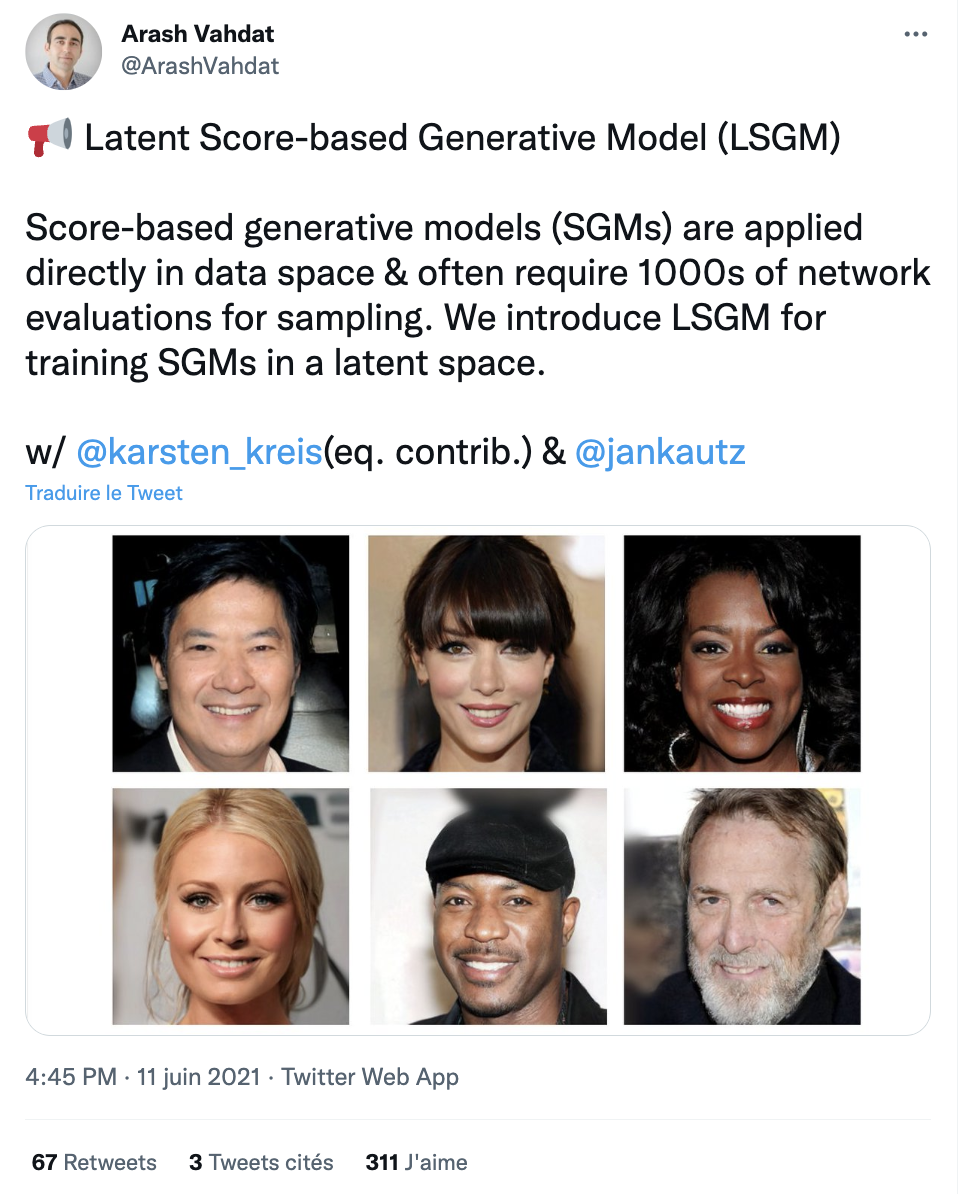
\includegraphics[width=.85\textwidth]{figures/impact_scholar/cont_diff_tweet.png}
%     \caption{}
%     \label{fig:cont_tweet}
%   \end{subfigure}
%   \begin{subfigure}[b]{.48\textwidth}
%     \centering
%     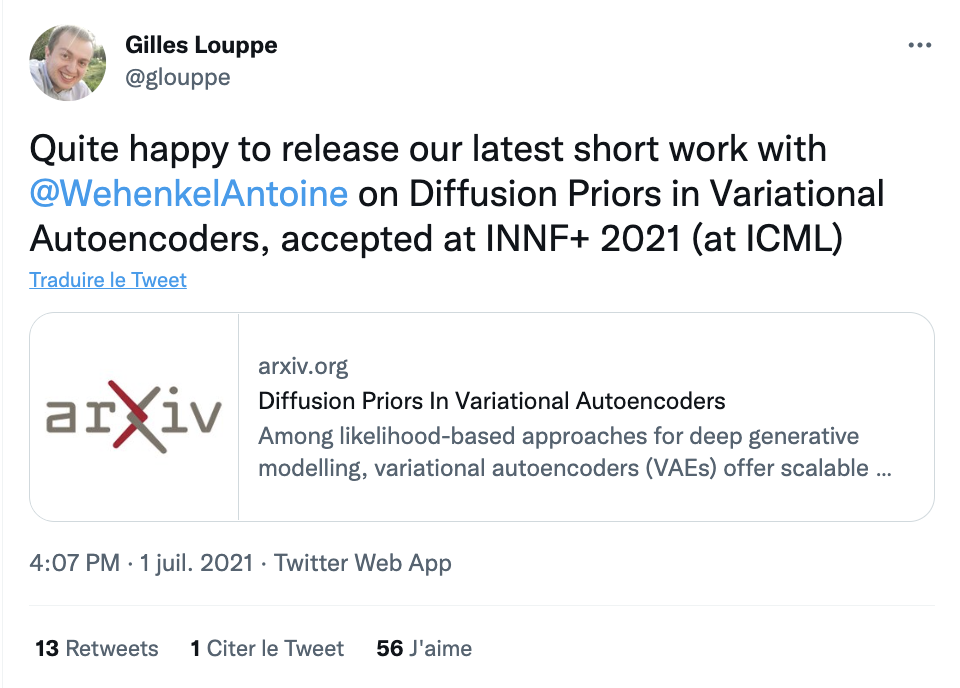
\includegraphics[width=.9\textwidth]{figures/impact_scholar/discret_diff_tweet.png}
%     \caption{}
%     \label{fig:discrete_tweet}
%   \end{subfigure}
%   \caption{Tweets advertising (\textbf{a}) continuous-time diffusion models in the latent space from \citet{vahdat2021score} (\textbf{b}) discrete-time diffusion models in the latent space.}
% \end{figure*}
